\documentclass[journal]{IEEEtran}
\usepackage[a5paper, margin=10mm]{geometry}
%\usepackage{lmodern} % Ensure lmodern is loaded for pdflatex
\usepackage{tfrupee} % Include tfrupee package


\setlength{\headheight}{1cm} % Set the height of the header box
\setlength{\headsep}{0mm}     % Set the distance between the header box and the top of the text


%\usepackage[a5paper, top=10mm, bottom=10mm, left=10mm, right=10mm]{geometry}

%
\usepackage{gvv-book}
\usepackage{gvv}
\setlength{\intextsep}{10pt} % Space between text and floats

\makeindex

\begin{document}
\bibliographystyle{IEEEtran}
\onecolumn
\newpage
\title{2023 February 1 Shift 2}
\author{AI24BTECH11004-Bheri Sai Likith Reddy}
\maketitle
\section{SECTION-A}

\begin{enumerate}
       \item The figure shows three glasses $P,Q$ and $R$ with water and floating ice cube. Glass $P$ has a solid ice cube, glass $Q$ has an air bubble. After the ice cube melts, the level of water in glasses $P,Q$ and $R$, respectively:
      \begin{figure}[ht!]
	    \centering
	    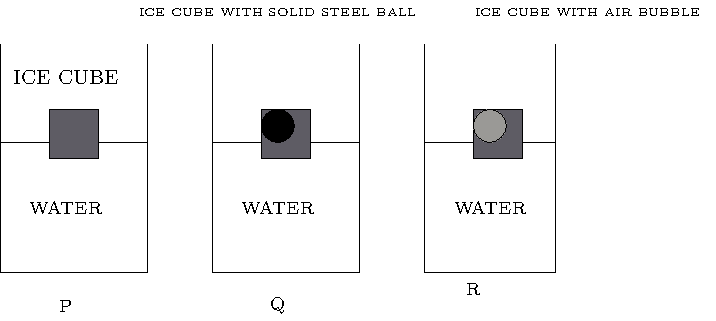
\includegraphics[width=0.5\linewidth]{fig/fig1.pdf}
	\end{figure}
       \begin{enumerate}
           \item remains same, increases, and decreases
           \item increases, decreases, and increases
           \item remains same, decreases, and decreases
           \item remains same, decreases, and increases
       \end{enumerate}
       \item To estimate aerodynamic loads on an aircraft flying at $100km/h$ at standard sea-level conditions, a one-fifth scale model is tsted in a varibel-density wind tunnel ensuring similarity of inertial and viscous forces. The pressure used in the wind runnel is $10$ times the atmospheric pressure. Assuming ideal gas law to hold and the same temperature conditions in model and prototype, the velocity needed in the wind tunnel test-section is \rule{1cm}{0.15mm}
       \begin{enumerate}
           \item $25km/h$
           \item $50km/h$
           \item $100km/h$
           \item $20km/h$
       \end{enumerate}
       \item The figure shows schematic of a set-up for visualization of non-uniform density field in the test section o fa supersonic wind tunnel. This technique of visualization of high speed flows is known as: 
\begin{figure}[ht!]
	    \centering
	    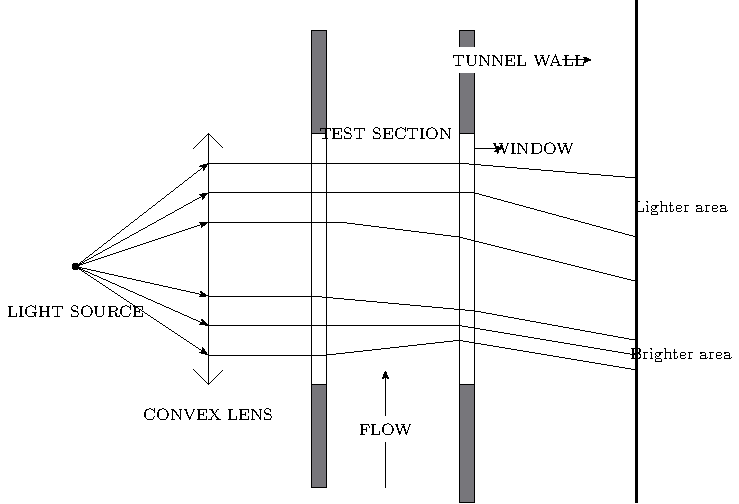
\includegraphics[width=0.5\linewidth]{fig/fig2.pdf}
	\end{figure}    
		\begin{enumerate}
           \item schlieren 
           \item interferometry
           \item shadowgraph
           \item holography
       \end{enumerate}
	\item For a conventional fixed-wing aicraft in a $360^\circ$ inverted vertical loop maneuver, what is the load factor \brak{n} at the topmost point of the loop? Assume the flight to be steady at the topmost point.
               \begin{enumerate}
			        \begin{multicols}{4}  
		       \item $n=1$
		       \item $n<1$
		       \item $n=-1$
		       \item $n>-1$
                    \end{multicols}   
	       \end{enumerate}	
\textbf{The next 5 question sare multiple select queestions and carry TWO mark each}
       \item Which of the following statement\brak{s} is/are true about the function defined as $f\brak{x} = e^{-x}\abs{\cos x} \text{ for } x>0 $?
             \begin{enumerate}
                 \item Differentiable at $x=\frac{\pi}{2}$
                 \item Differentiable at $x=\pi$
                 \item Differentiable at $x=\frac{3\pi}{2}$
                 \item Continuous at $x=2\pi$
             \end{enumerate}
	\item  A two degree of freedom spring-mass system undergoing free vibration with generalized coordinates $x_1$ and $x_2$ has natural frequencies $\omega_1=233.9rad/s$ and $\omega_2=324.5rad/s$, respectively. The corresponding mode shapes are $\phi_1=\myvec{1\\-3.16}$ and $\phi_2=myvec{1\\3.16}$. If the system is disturbed with certain deflection sand zero initial velocities, then which of the following statement\brak{s} is/are true?
		\begin{enumerate}
			\item An initial deflection of $ x_1\brak{0}=6.32cm$ and $x_2\brak{0}=-3.16cm$ would make the system oscillate with only the second natural frequency. 
			\item An initial deflection of $ x_1\brak{0}=2cm$ and $x_2\brak{0}=-6.32cm$ would make the system oscillate with only the first natural frequency. 
			\item  An initial deflection of $ x_1\brak{0}=62cm$ and $x_2\brak{0}=-2cm$ would make the system oscillate with a linear combination of first and second natural frequencies. 
	        \item  An initial deflection of $ x_1\brak{0}=1cm$ and $x_2\brak{0}=-6.32cm$ would make the system oscillate with only the first natural frequency. 
        	\end{enumerate}
	\item A shock moving into a stationary gas can be transformedd to a stationary shock by a change in reference frame, as shown in the figure. Which of the following is/are true relation the flow properties in the two  reference frames?
		\newpage
\begin{figure}[ht!]
	    \centering
	    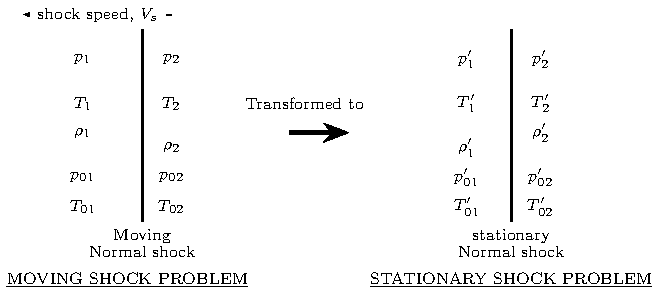
\includegraphics[width=0.5\linewidth]{fig/fig3.pdf}
	\end{figure}  
		\begin{enumerate}
             \item $T_1'>T_1,T_{01}'>T_{01},p_{01}'>p_{01},\rho_2'>\rho_1'$
             \item $T_1'=T_1,T_{2}'<T_{01},p_{01}'>p_{01},\rho_2'=\rho_2$
             \item $T_1'<T_1,p_{1}'>p_{1},p_{01}'>p_{01},\rho_2'>\rho_1$
             \item $T_1'=T_1,p_{2}>p_{01},T_{01}'>T_{01},p_{01}'>p_{10}$
         \end{enumerate}
	\item For a conventional fixed-wing aircraft, which of rhe following statements are true?
          \begin{enumerate}
              \item Making $C_{m_\alpha}$ more negative leads to an increase in the frequency of its short-period mode.
              \item Making $C_{m_q}$ more negative leads to a decreased damping off the short-period mode.
              \item The peimary contribution towards $C_{l_p}$ is from the aircraft wing.
              \item  Increase the size of he vertical fin leads to a higher yaw damping.
          \end{enumerate}
	\item Which of the folloing statement\brak{s} is/are true?
         \begin{enumerate}
             \item Service ceiling is higher than absolute ceiling for a piston-propeller aircraft.
             \item For a given aircraft, teh stall speed increase with increase in altitude.
             \item Everything else remaining the same, a tailwind increase the range of an aircraft.
             \item For a jet aircraft comstrained ro fly at constant altitude, there exists an altitude where its range is maximum.
         \end{enumerate}
	\item A conventional fixed-wing aircraft, with a horizontal tail and vertical fin, in steady and level flight is subjected to small perturbations. Which of the following statement\brak{s} is/are true?
          \begin{enumerate}
              \item Vertical fin has a stabilizing effecgt on the lateral stabilithy of the aircraft.
              \item Vertical fin has a destabilizing effect on the directional stability of the aircraft.
              \item Presence of wing anhedral increase the lateral stability of the aircraft. 
              \item Horizontal tail has a stabilizing effect on the longitudinal static stability of the aircraft.
          \end{enumerate}
\textbf{The next 19 questions are Numerical answer type \brak{NAT}, carry TWO mark each (no negative marks)}
    \item The ratio of the product of eigenvalues to the sum of the eigenvalues of the given matrix
            \begin{align*}
                \myvec{3&1&2\\2&-3&-1\\1&2&1}
            \end{align*}
            is \rule{1cm}{0.15mm} \brak{\text{round off to nearest integer}}
	\item The definite integral $\int_1^5x^2dx$ is evaluated using four equal interval by two methods-first by the trapezoidal rule and then by the Simpson's onw-third rule. The absolute value of the difference between the two calculations is \rule{1cm}{0.15mm} (round off to two decimal places).
	\item  The deflection $y$ of a certain beam of length $l$ and uniform weight per unit length $w$, is given as $y=\frac{w}{48EI}\brak{2x^4-3lx^3+l^3x}$, where $x$ is the distance from the point of support andd $EI$ us a constant. The non-dimensional location $\frac{x}{l}$, where the deflection of the beam is maximum,is \rule{1cm}{0.15mm} (round off to two decimal places).  
	
\end{enumerate}	
\end{document}

